\label{sec:2.4}
%\clearpage
%%%%%%%%%%%%%%%%%%%%%%%%%%%%%%%%%%%%%%%%%%%%%%%%%%%%%%%
% Lin and Prakash - LBL test setup
%%%%%%%%%%%%%%%%%%%%%%%%%%%%%%%%%%%%%%%%%%%%%%%%%%%%%%%
The ASIC testing at LBNL uses the CTS to cool the ColdADC to cryogenic temperature. A single board solution was 
developed by LBNL to test the ColdADC. The test board accommodates one ColdADC bare die, wire bonded to the board. 
The board is divided into cold and warm sections with an empty strip of PCB in between to clamp the board to CTS.
The cold section of the PCB contains the ColdADC die and four low noise LDOs.
Power supply distribution circuitry, Spartan 6 FPGA,  80MHz oscillator for clocking 
the FPGA, and the Raspberry PI are in the warm section of the test board. Analog inputs to 
the ColdADC are supplied by 16 edge-mount SMA connectors. There are two additional edge-mount SMA connectors 
to supply test inputs directly to the ADC-core. Eight-pin standard header connector is available if there is 
a need to bypass the ColdADC LDOs and supply external VDDs directly to the ASIC.
The first version of the test board was used extensively to evaluate the ColdADC performance.  However, due to the small 
block-RAM size of the FPGA, the ADC data cannot be streamed continuously to the Raspberry PI. Thus makes
data collection a time consuming process. Another limitation is that the inputs to the ColdADC can only be single-ended due 
the space constraints for mounting the SMA connectors.

Recently, a version 2 of the test board was developed to improve data throughput and address some other limitations 
of the previous test board.  The new design is a three-board 
solution, which consists of a motherboard, a daughter card and an FPGA mezzanine board. The daughter card can either have a 
bare die or a packaged chip. A modular approach was taken so the same test setup 
can be used for the next iteration of the ColdADC V2 chip just by minor re-designing the Chip-On-Board (COB) daughter card. The V2 LBNL 
test board is shown in Figure \ref{fig:v2_board}. This test board, similar to the previous version, has cold and warm 
sections. The COB daughter card and the LDOs are at the bottom, in the cold section of the board. The power 
distribution circuitry, FPGA mezzanine board, and the Raspberry PI are in the warm section of the board. 
Four 8-pin Samtec 5.00 mm 50 Ohm Ganged Micro-Miniature RF Jack connectors are used to drive external 
differential or single ended analog inputs to the ColdADC.  

\begin{figure}[!ht]
\centering
 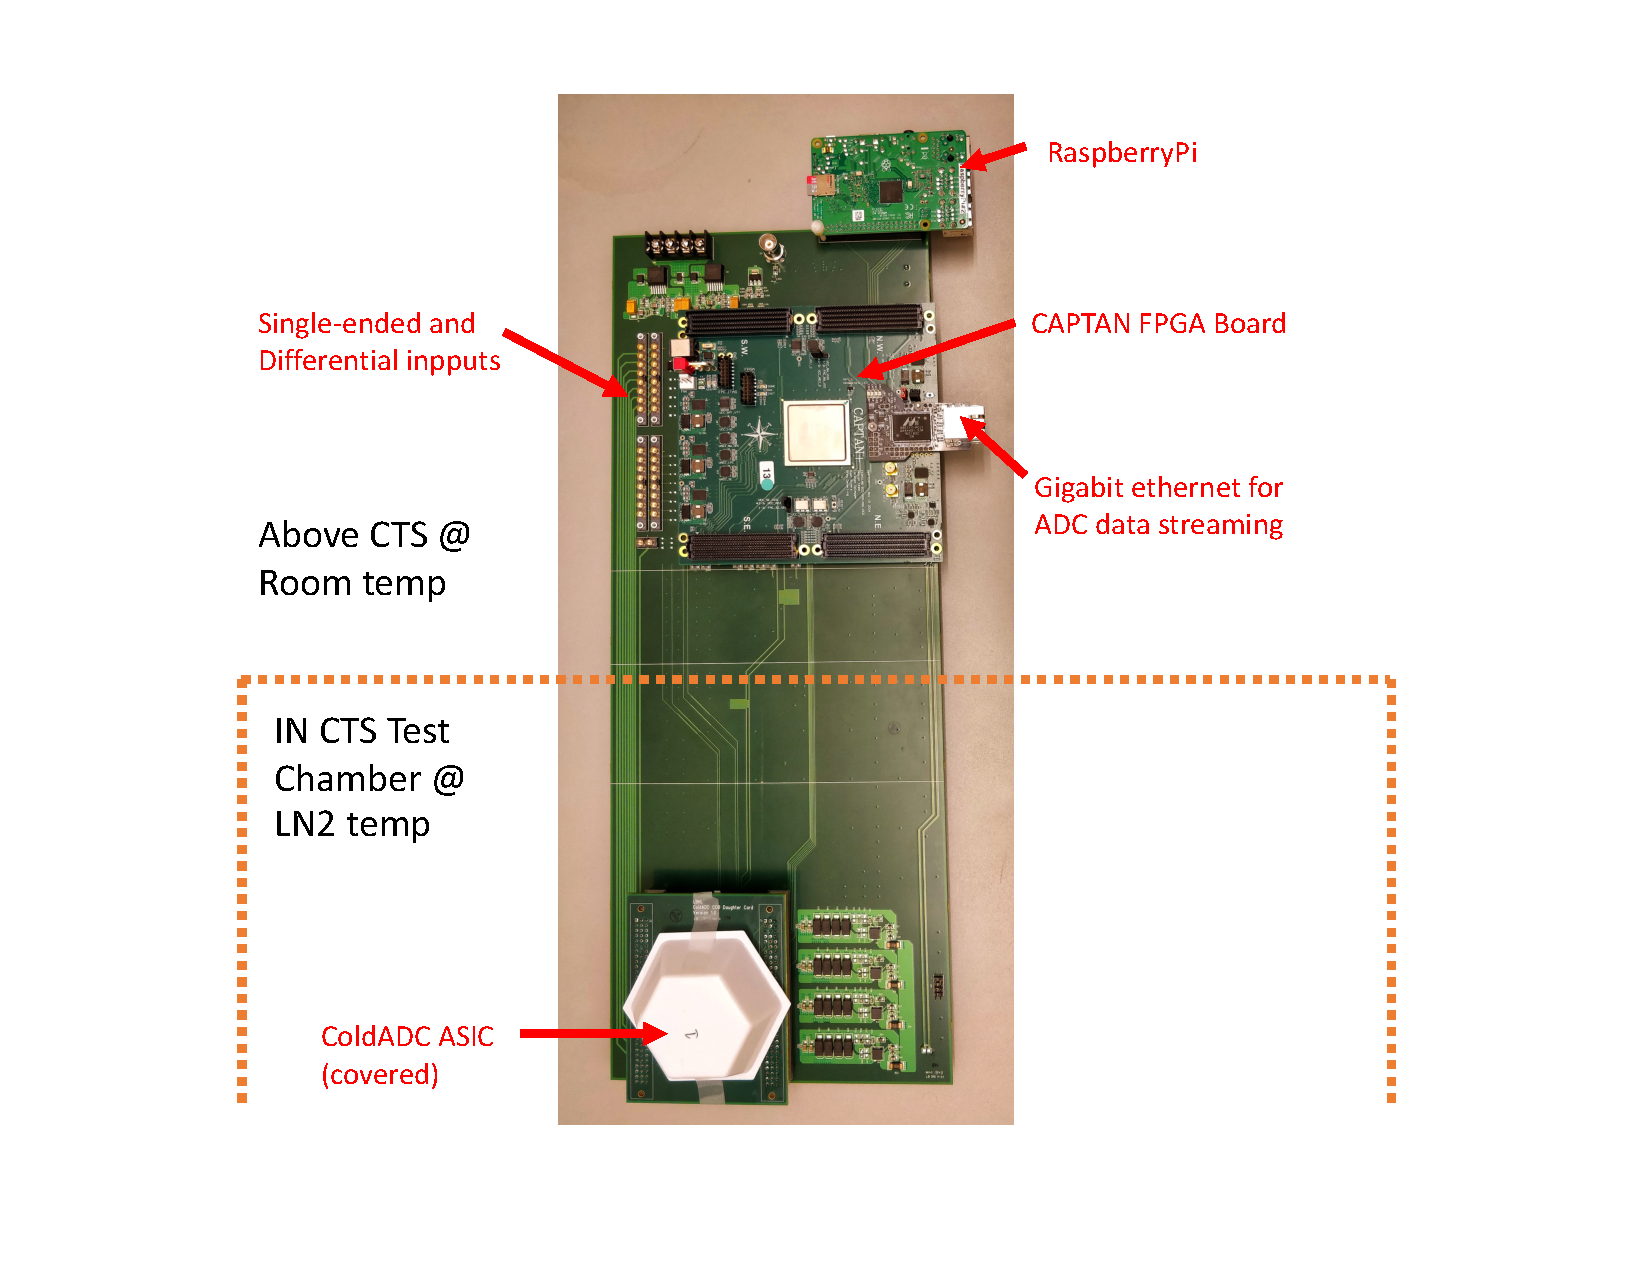
\includegraphics[width=0.85\linewidth]{figures/prakash_fig/TestBoard2_CTS.pdf}
  \caption[LBNL ColdADC Testboard]{Version 2 LBNL ColdADC Testboard}
  \label{fig:v2_board}
\end{figure}


